\colorlet{species background color}{black!15}
\tikzset{
    x={1pt},
    y={-1pt},
    species background/.style={
        fill=species background color,
        draw=species background color,
        line width={1pt},
    },
    species label/.style={
        font=\bfseries,
        midway,
        anchor=north,
        align=center,
        yshift=-10,
    },
    branch/.style={
        draw={#1},
        line width={0.5pt},
    },
    transfer branch/.style={
        branch={#1},
        -Stealth,
    },
    loss/.style={
        draw={#1}, cross out, thick,
        line width={0.5pt},
        inner sep=0pt,
        outer sep=0pt,
        minimum width={3},
        minimum height={3},
    },
    extant gene/.style 2 args={
        circle, fill={#1},
        outer sep=0pt, inner sep=0pt,
        minimum size={3},
        label={
            [font={\strut\color{#1}},
                align=center,
                inner xsep=0pt, inner ysep=2pt,
                outer xsep=0pt, outer ysep=0pt]
            below:#2
        },
    },
    extant gene/.default={black}{},
    branch node/.style={
        draw={#1}, fill={species background color!50!white},
        align=center,
        font={\color{#1}},
        outer sep=0pt, inner xsep=0pt, inner ysep=2pt,
        line width={0.5pt},
    },
    branch node/.default={black},
    speciation/.style={
        branch node={#1}, rectangle, rounded corners,
        inner xsep=4pt,
        minimum width={8},
        minimum height={8},
    },
    duplication/.style={
        branch node={#1}, rectangle,
        inner xsep=4pt,
        minimum width={8},
        minimum height={8},
    },
    horizontal gene transfer/.style={
        branch node={#1}, chamfered rectangle,
        chamfered rectangle sep={8 / 2.4},
        inner xsep=2pt,
        inner ysep=-1pt,
        minimum width={8},
        minimum height={8},
    },
}
\definecolor{reccolor0}{HTML}{000000}
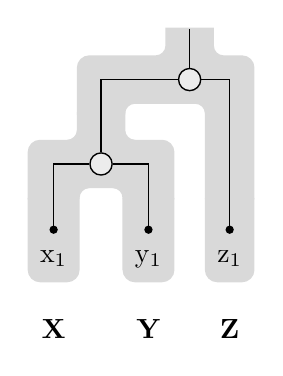
\begin{tikzpicture}
% background
\path[species background] (17.763,30.5) [rounded corners={4pt}] -- (17.763,10) -- (49.776,10) [sharp corners] -- (49.776,0) -- (66.276,0) [rounded corners={4pt}] -- (66.276,10) -- (80.949,10) [sharp corners] -- (80.949,61.0) -- (64.026,61.0) [rounded corners={4pt}] -- (64.026,26.5) -- (34.263,26.5) [sharp corners] -- (34.263,30.5) -- cycle;
\path[species background] (0,61.0) [rounded corners={4pt}] -- (0,40.5) -- (17.763,40.5) [sharp corners] -- (17.763,30.5) -- (34.263,30.5) [rounded corners={4pt}] -- (34.263,40.5) -- (52.026,40.5) [sharp corners] -- (52.026,61.0) -- (34.263,61.0) [rounded corners={4pt}] -- (34.263,57.0) -- (17.763,57.0) [sharp corners] -- (17.763,61.0) -- cycle;
\path[species background, rounded corners={4pt}] (0,61.0) -- (0,91.0) -- node[species label] {X} (17.763,91.0) -- (17.763,61.0);
\path[species background, rounded corners={4pt}] (34.263,61.0) -- (34.263,91.0) -- node[species label] {Y} (52.026,91.0) -- (52.026,61.0);
\path[species background, rounded corners={4pt}] (64.026,61.0) -- (64.026,91.0) -- node[species label] {Z} (80.949,91.0) -- (80.949,61.0);
% gene branches
\path[branch={reccolor0}] (58.026,14) -- (58.026,0);
\path[branch={reccolor0}] (26.013,30.5) |- (53.776,18.25) (62.276,18.25) -| (72.4875,61.0);
\path[branch={reccolor0}] (26.013,44.5) -- (26.013,30.5);
\path[branch={reccolor0}] (8.8815,61.0) |- (21.763,48.75) (30.263,48.75) -| (43.1445,61.0);
\path[branch={reccolor0}] (8.8815,71.0) -- (8.8815,61.0);
\path[branch={reccolor0}] (43.1445,71.0) -- (43.1445,61.0);
\path[branch={reccolor0}] (72.4875,71.0) -- (72.4875,61.0);
% gene transfers
% events
\node[speciation={reccolor0}] at (58.026,18.25) {};
\node[speciation={reccolor0}] at (26.013,48.75) {};
\node[extant gene={reccolor0}{x\textsubscript{1}}] at (8.8815,72.5) {};
\node[extant gene={reccolor0}{y\textsubscript{1}}] at (43.1445,72.5) {};
\node[extant gene={reccolor0}{z\textsubscript{1}}] at (72.4875,72.5) {};
\end{tikzpicture}
